\documentclass[journal]{IEEEtran}

\usepackage{cite}
\usepackage{amsmath}
\interdisplaylinepenalty=2500
\usepackage{algorithm}
\usepackage[noend]{algpseudocode}
\usepackage{array}
\usepackage{graphicx}
\usepackage{float}

% correct bad hyphenation here
\hyphenation{}


\begin{document}
\title{Particle Swarm Optimization}

\author{Wilbert~Pumacay,~\textit{Catholic University San Pablo},~wilbert.pumacay@ucsp.edu.pe\\
        Gerson~Vizcarra,~\textit{Catholic University San Pablo},~gerson.vizcarra@ucsp.edu.pe}

% make the title area
\maketitle

\begin{abstract}
Heuristics-based swarm algorithms emerged as a powerful family of optimization techniques, inspired by the collective behavior of social animals. Particle Swarm Optimization (PSO) , part of this family, is known to solve large-scale nonlinear optimization problems using particles as set of candidate solutions. In this paper we test the PSO on 3 common benchmarks functions and compare it with the results from other metaheuristics using the Wilcoxon rank sum test. 
\\
\\
We also implemented a parallel version of the algorithm in CUDA to speed up the optimization process and allow more particles to be used.
\end{abstract}

\begin{IEEEkeywords}
Metaheuristics, Particle Swarm Optimization, Convergence Behavior, CUDA.
\end{IEEEkeywords}


\section{Introduction}


\section{ Particle Swarm Optimization (PSO) }
\subsection{Basic concepts}
Particle Swarm Optimization, first introduced by Kennedy and Eberhart \cite{Kennedy1995} is a stochastic optimization technique htat is based on two fundamental diciplines·\cite{delValle2008}: social science and computer science. In addition, PSO uses the swarm intelligence concept: the collective behavior of unsophisticated agents that are interacting locally with their environment create coherent global functional patterns.

\subsubsection{ Social concepts }
Human intelligence resulting of social interaction consist in evaluate, compare and imitate to others, as well to learn of experience allow to humans to adapt to the environment and find optimal patterns of behavior

\subsubsection{ Swarm intelligence }
Swarm intelligence can be described by considering principles, this principles are based on biological agents; according to \cite{Garnier2007} there are four main principles.
\begin{enumerate}
    \item Coordination: Information is shared among the agents.
    \item Collaboration: Agents can do different tasks in parallel.
    \item Deliberation: Agents can determine priorities if they have more than one option.
    \item Cooperation: Agents combine their efforts to successfully solve a problem.
\end{enumerate}

\subsubsection{ Computational Characteristics }



\subsection{PSO in Real Number Space}


\subsection{Implementation details}

\begin{figure*}
\centering
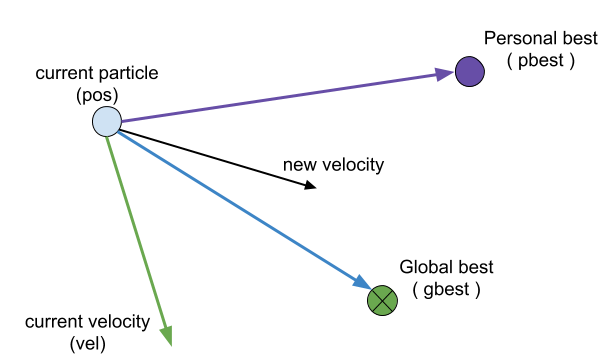
\includegraphics[width=4.0in]{_img/img_PSO_overview.png}
\caption{PSO overview}
\end{figure*}

For the CPU implementation we followed this simple variation of the asynchronous PSO algorithm :

\begin{algorithm*}
    \caption{Particle Swarm Optimization - Asynchonous Serial Version}\label{alg:PSOcpu}
    \begin{algorithmic}[1]
        \State $\textbf{In}: \textit{objFunction, populationSize, w, $c_{1}$, $c_{2}$, k, dimensions, domain}$
        \State $\textbf{Out}: \textit{Solution optima } P_{g.cost}$
        \State $vMin = -k * ( domain.max - domain.min ) / 2.0$
        \State $vMax =  k * ( domain.max - domain.min ) / 2.0$
        \State $P_{g.pos} = \textit{zeros( dimensions )}$ \Comment{Position that gives best cost}
        \State $P_{g.cost} = Inf$ \Comment{Best cost so far}
        \\
        \State $Particles=\lbrace \rbrace$ \Comment{Empty array of particles}
        \For {$i=1$ {\bfseries to} $PopulationSize$} \Comment{Particles Initialization}
            \State $p = \textbf{Particle()}$
            \State $p.pos = \textbf{randUniform( domain )}$
            \State $p.vel = \textbf{zeros( dimensions )}$
            \State $p.cost = \textbf{objFunction( p.pos )}$
            \State $p.bestpos = p.pos$
            \State $p.bestcost = p.cost$
            \If {$p.cost \leq P_{g.cost}$}
                \State $P_{g.cost} = p.cost$
                \State $P_{g.pos} = p.pos$
            \EndIf
        \EndFor
        \\
        \While {$\textit{ !stopCondition() }$} \Comment{Optimization process}
            \For {$p$ {\bfseries in} $Particles$}
                \State $p.vel = w * p.vel + 
                                c_{1} * ( p.bestpos - p.pos ) + 
                                c_{2} * ( P_{g.pos} - p.pos )$ \Comment{Velocity update}
                \State $p.vel = \textbf{ClampVector}\textit{( p.vel, vMin, vMax )}$
                \State $p.pos = p.pos + p.vel$ \Comment{Position update}
                \State $p.pos = \textbf{ClipPosition}\textit{( p.pos, domain )}$
                \\
                \If {$p.cost \leq p.bestcost$}
                    \State $p.bestcost = p.cost$ \Comment{Update personal best}
                    \State $p.bestpos = p.pos$
                    \If {$p.cost \leq P_{g.cost}$}
                        \State $P_{g.cost} = p.cost$ \Comment{Update global best}
                        \State $P_{g.pos} = p.pos$
                    \EndIf
                \EndIf
            \EndFor
        \EndWhile
        \\
        \Return $P_{g.cost}$
    \end{algorithmic}
\end{algorithm*}

For the GPU implementation we followed the same variation of the PSO algorithm in a synchronous way, by making the comparison with the global best outside of the particles update loop :

\begin{algorithm*}
    \caption{Particle Swarm Optimization - Synchonous Parallel Gpu Version}\label{alg:PSOgpu}
    \begin{algorithmic}[1]
        \State $\textbf{In}: \textit{objFunction, populationSize, w, $c_{1}$, $c_{2}$, k, dimensions, domain}$
        \State $\textbf{Out}: \textit{Solution optima } P_{g.cost}$
        \State $vMin = -k * ( domain.max - domain.min ) / 2.0$
        \State $vMax =  k * ( domain.max - domain.min ) / 2.0$
        \State $P_{g.pos} = \textit{zeros( dimensions )}$ \Comment{Position that gives best cost}
        \State $P_{g.cost} = Inf$ \Comment{Best cost so far}
        \\
        \State $hostParticles = \lbrace \rbrace$
        \State $deviceParticles = \lbrace \rbrace$
        \State $\textbf{GpuCreateParticles}\textit{( hostParticles, deviceParticles, objFunction, populationSize, dimensions, domain )}$
        \State $\textbf{GpuInitParticles}\textit{( hostParticles, deviceParticles, objFunction )}$
        \\
        \While {$\textit{ !stopCondition() }$} \Comment{Optimization process}
            \State $\textbf{GpuUpdateParticles}\textit{( hostParticles, deviceParticles, w, $c_{1}$, $c_{2}$, k )}$s
            \For {$p$ {\bfseries in} $hostParticles$}
                \If {$p.cost \leq P_{g.cost}$}
                    \State $P_{g.cost} = p.cost$ \Comment{Update global best}
                    \State $P_{g.pos} = p.pos$
                \EndIf
            \EndFor
        \EndWhile
        \Return $P_{g.cost}$
    \end{algorithmic}
\end{algorithm*}

\begin{algorithm*}
    \caption{Particle Swarm Optimization - GpuUpdateParticles}\label{alg:PSOgpu_kernel_updateparticles}
    \begin{algorithmic}[1]
        \State $\textbf{In}: \textit{deviceParticles, coreIndx, w, $c_{1}$, $c_{2}$, k, $P_{g}$}$
        \State $p = \textbf{getDeviceParticle}\textit{( coreIndx )}$
        \State $p.vel = w * p.vel + 
                        c_{1} * ( p.bestpos - p.pos ) + 
                        c_{2} * ( P_{g.pos} - p.pos )$ \Comment{Velocity update}
        \State $p.vel = \textbf{ClampVector}\textit{( p.vel, vMin, vMax )}$
        \State $p.pos = p.pos + p.vel$ \Comment{Position update}
        \State $p.pos = \textbf{ClipPosition}\textit{( p.pos, domain )}$
        \\
        \If {$p.cost \leq p.bestcost$}
            \State $p.bestcost = p.cost$ \Comment{Update personal best}
            \State $p.bestpos = p.pos$
        \EndIf
    \end{algorithmic}
\end{algorithm*}

\begin{figure*}
\centering
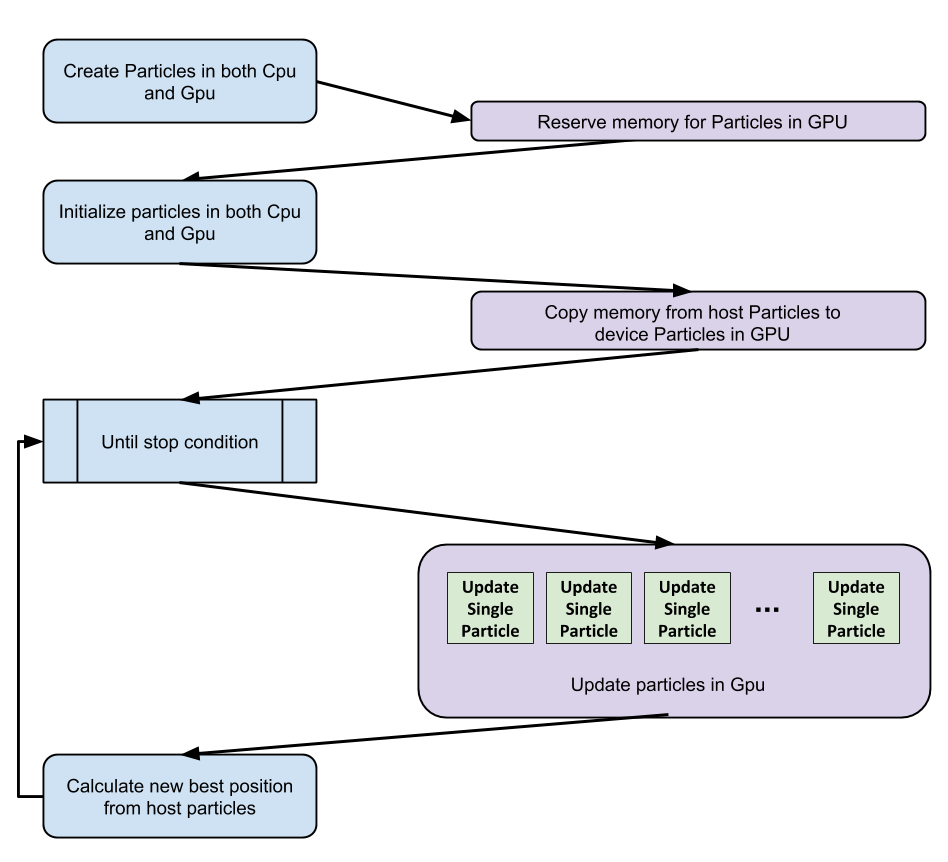
\includegraphics[width=4.0in]{_img/img_PSO_algorithm_gpu.png}
\caption{PSO algorithm in GPU}
\end{figure*}

\section{Results}


\section{Conclusions and Future improvements}


\IEEEtriggeratref{8}

% references section
\begin{thebibliography}{1}

\bibitem{Kennedy1995}
  James Kennedy and Russell Eberhart. \\
  \textit{Particle Swarm Optimization.} - 1995
\\
\bibitem{Garnier2007}
  Simon Garnier, Jacques Gautrais, Guy Theraulaz\\
  \textit{The biological principles of swarm intelligence.} - 2007
\\
\bibitem{delValle2008}
  Yamille del Valle, Ganesh Kumar, Salman Mohagheghi, Jean Hernandez, Ronald Harley\\
  \textit{Particle Swarm Optimization: Basic Concepts, Variants and Applications in Power Systems.} - 2008
\\
\bibitem{CameraCalibration1}
  Zhengyou Zhang \\
  \textit{A Flexible New Technique for Camera Calibration.} - 2000
\\
\bibitem{IntegralImageThresholding}
  Derek Bradley, Gerhard Roth \\
  \textit{Adaptive Thresholding Using the Integral Image.} - 2011

\end{thebibliography}


\end{document}
